\documentclass[aps,showpacs,superscriptaddress,twocolumn,pra]{revtex4}
\usepackage{txfonts}
\usepackage{stmaryrd}
\usepackage{mathrsfs}

\usepackage{amsmath}
\usepackage{amsfonts}
\usepackage{amssymb}
\usepackage{graphicx}
\usepackage{dcolumn}
\usepackage{bm}
\usepackage[colorlinks=true,dvipdfm]{hyperref}

\setcounter{MaxMatrixCols}{10}

\renewcommand{\textfraction}{0.15}
\renewcommand{\topfraction}{0.85}
\renewcommand{\bottomfraction}{0.65}
\renewcommand{\floatpagefraction}{0.60}


\begin{document}
\title{Experimental Implementation of a Quantum Random-Walk Search Algorithm Using Strongly Dipolar Coupled Spins}
\author{Dawei Lu}
\affiliation{Hefei National Laboratory for Physical Sciences at
Microscale and Department of Modern Physics, University of Science
and Technology of China, Hefei, Anhui, 230026, China}
\author{Jing Zhu}
\affiliation{Hefei National Laboratory for Physical Sciences at
Microscale and Department of Modern Physics, University of Science
and Technology of China, Hefei, Anhui, 230026, China}
\affiliation{Department of Physics $\&$ Shanghai Key Laboratory for
Magnetic Resonance, East China Normal University�� Shanghai 200062}
\author{Ping Zou}
 \affiliation{Laboratory of Quantum Information Technology, ICMP and SPTE, South China Normal University, Guangzhou 510006, China}
\author{Xinhua Peng}
 \affiliation{Hefei National Laboratory for Physical Sciences at
Microscale and Department of Modern Physics, University of Science
and Technology of China, Hefei, Anhui, 230026, China}
\author{Yihua Yu}
 \affiliation{Department of Physics $\&$ Shanghai Key Laboratory for
Magnetic Resonance, East China Normal University�� Shanghai 200062}
\author{Shanmin Zhang}
 \affiliation{Department of Physics $\&$ Shanghai Key Laboratory for
Magnetic Resonance, East China Normal University�� Shanghai 200062}
\author{Qun Chen}
 \affiliation{Department of Physics $\&$ Shanghai Key Laboratory for
Magnetic Resonance, East China Normal University�� Shanghai 200062}
\author{Jiangfeng Du}
 \email{djf@ustc.edu.cn}\affiliation{Hefei National Laboratory for Physical Sciences at
Microscale and Department of Modern Physics, University of Science
and Technology of China, Hefei, Anhui, 230026, China}

\begin{abstract}
An important quantum search algorithm based on the quantum random
walk performs an oracle search on a database of N items with
$\emph{O}(\sqrt{\emph{N}})$ calls, yielding a speed-up  similar to
the Grover's quantum search algorithm. The algorithm was implemented
on a quantum information processor of three-qubit liquid-crystal
nuclear magnetic resonance in the case of finding 1-out-of-4, and
the diagonal elements' tomography of all the final density matrices
was completed with comprehensible one-dimensional NMR spectra. The
experimental results agree well with the theoretical predictions.
\end{abstract}

\pacs{03.67.Lx, 05.40.Fb, 76.60.2k}\maketitle
\subsection*{I. Introduction}

Quantum computation has attracted much attention for the past decade
as it is believed that quantum computers can efficiently solve problems which are
intractable to classical computers. The computation tasks are
rendered by algorithms. Since Shor's remarkable factoring algorithm
\cite{Shor}, many quantum algorithms have been proposed. The
algorithms presented early are mainly based on the quantum Fourier
transform \cite{Shor} and Grover's search algorithm \cite{Grover}.
Later two alternative trends have entered into the field, the
adiabatic quantum algorithms \cite{Farhi} and quantum random walk
\cite{Aharonov,Farhi and Gutmann,Ambainis and Back,Childs and
Farhi,Childs and Cleve,Brun,Ambainis,Farhi and Goldstone,Childs}. In
this paper, we focus on the quantum-walk based search algorithm.

Since the classical random walk is a useful tool for developing
classical algorithms, the quantum random walk has been introduced as
a potential method to formulate quantum algorithms. There are two
distinct models, the continuous-time model and discrete-time model.
The continuous-time model defines a Hamiltonian which acts continuously on the system to drive the quantum random walk. The discrete-time model
requires an extra coin register and defines a two-step procedure
consisting of a quantum coin flip followed by a coin-controlled walk
step. Investigations show that quantum random walks have notable
different features to their classical counterparts
\cite{Aharonov,Farhi and Gutmann}. These features may be used for
designing quantum algorithms. Some relevant algorithms have been
discovered with remarkable speedup over classical computation
\cite{Childs and Cleve,Shenvi}. The quantum search algorithm based
on the quantum random walk proposed by Shenvi, Kempe, and Whaley
(the SKW algorithm) \cite{Shenvi} is one of the novel algorithms,
for performing an oracle search on a database of \emph{N} items with
$\emph{O}(\sqrt{\emph{N}})$ calls, where \emph{N} is the size of the
search space. Despite of a similar speed-up to the Grover's quantum
search algorithm, the SKW algorithm is important as there are
situations when the diffusion step of Grover's algorithm can not be
implemented efficiently. Various optimizations and improvements of
the SKW algorithm have also been proposed in recent years
\cite{Ambainis and Kempe,Tulsi,Reitzner,Chandrashekar,Potocek},
which can reduce the complexity and increase the search capability
to a certain extent.

Some experiments about quantum random walk have been implemented in
various physical systems under both continuous-time and
discrete-time conditions \cite{Travaglione,Du,Ryan,Chandrashekar},
but as much as we know, no experiments about the algorithms based on
quantum random walk have been reported. In this paper, we
experimentally demonstrate the 1-out-of-4 case of the SKW algorithm
\cite{Shenvi} and show its superiority over classical algorithms.
The experiments are performed on a quantum information processor of
liquid-crystal nuclear magnetic resonance, with a strongly dipolar
coupled Hamiltonian \cite{Mahesh,Henry,Zhang}. More details are described in Section III.


\subsection*{II. Algorithm}

First we give an overview of the original algorithm. Consider the unstructured search problem: given a function $\emph{f}\left(\emph{x}\right)$, $\emph{f}\left(\emph{x}\right)=1$ if $\emph{x}=\emph{a}$, otherwise $\emph{f}\left(\emph{x}\right)=0$. The goal is to find \emph{a}, where $0\leqslant \emph{a}\leqslant 2^n-1$. It is equivalent to search for a single marked node among the $\emph{N}=2^n$ nodes on the n-cube.

The discrete-time random walk can be described by the repeated
application of a unitary evolution operator $U$. $U$ can be divided
into two parts $U=SC$, where $S$ is a permutation matrix which
performs a controlled shift based on the state of the coin space,
and $C$ is a unitary matrix corresponding to "flipping" the quantum
coin. To search for the node, SKW introduces an oracle whose
function is determined by the coin operator. The oracle will act by
applying a marking coin $C_1$ to the marked node and the original
coin $C_0$ to the unmarked nodes. This new coin operator is named
$C'$. Then the perturbed unitary evolution operator $U'$ is given by
$U'=SC'$ (see Fig.\ref{net}). After applying $U'$ for
$t_{f}=\frac{\pi}{2}\sqrt{2^n}$ times, we will gain the marked state
with probability $\frac{1}{2}-O(n)$ by measurement.

\begin{figure}[h] \centering
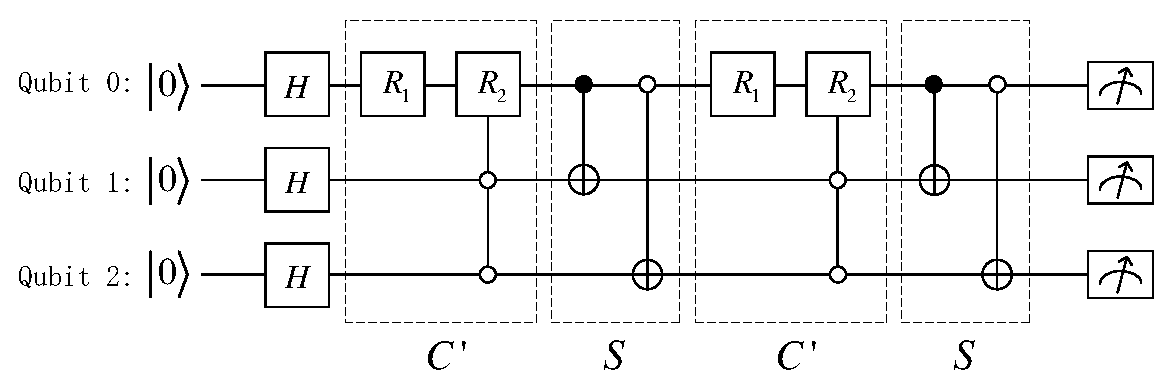
\includegraphics[width=\columnwidth]{net.eps}
\caption{\footnotesize{Quantum network for the algorithm of
1-out-of-4 searching, with the target state being $\left\vert 00
\right\rangle_{12}$. Qubit 0 is the "coin qubit" while qubit 1 and 2 are "database qubits".
The Hadamard gates are applied to pruduce an equal superposition over all the computational basis.
The black dot represents 1-control gate while
the white dot reversely. The purpose of $C'$ is to implement
$C_1=R_x^0(\pi/2)$ (rotating qubit 0 around the \emph{x} axis by
angle $\pi/2$) when the "database" is $\left\vert 00
\right\rangle_{12}$ and $C_0=R_x^0(3\pi/2)$ otherwise. It is
equivalent to be replaced by $R_1=R_x^0(3\pi/2)$ and
$R_2=R_x^0(-\pi)$. The two controlled-not gates are inverting qubit
1 if qubit 0 is $\left\vert 1 \right\rangle_{0}$ and inverting qubit
2 if qubit 0 is $\left\vert 0 \right\rangle_{0}$, respectively. The
measurement is all the populations', namely, diagonal elements'
reconstruction. Similar circuits can be obtained straightforwardly
for other target states. For instance if the goal is $\left\vert 10
\right\rangle_{12}$, we need only change the controlled condition of
the three-body-interaction gate to state $\left\vert 10
\right\rangle_{12}$.}}\label{net}
\end{figure}

When $n=2$, three qubits are needed to demonstrate the algorithm.
One qubit is used as the "coin" (referred as the "coin qubit",
labeled by qubit 0), while the other two are used as the database
(referred as the "database qubits", labeled by qubit 1 and 2). The
target state is $\left\vert \tau\sigma \right\rangle_{12} =
\left\vert \tau \right\rangle_{1}\otimes\left\vert \sigma
\right\rangle_{2} \left(\tau,\sigma=0,1 \right)$ out of the four
computational basis ${\left\vert 00 \right\rangle_{12},\left\vert 01
\right\rangle_{12},\left\vert 10 \right\rangle_{12},\left\vert 11
\right\rangle_{12}}$. The 1-out-of-4 algorithm is implemented as the
network shown in Fig.\ref{net}. Suppose
the initial state is $\left\vert 000 \right\rangle$.

(i) Prepare the state
\begin{equation} \label{initial}
\left\vert \psi_{i} \right\rangle=\frac{\left\vert 0 \right\rangle_0+\left\vert 1 \right\rangle_0}{\sqrt{2}}\otimes\frac{\left\vert 0 \right\rangle_1+\left\vert 1 \right\rangle_1}{\sqrt{2}}\otimes\frac{\left\vert 0 \right\rangle_2+\left\vert 1 \right\rangle_2}{\sqrt{2}},
\end{equation}
which is exactly an equal superposition over all the computational basis. It is simple to do this by applying a Hadamard operation to every qubit.

(ii) Perform the unitary operation on the "coin qubit"
depending on the state of "database qubits", namely,
$C_1=R_x^0(\pi/2)=e^{-i\pi\sigma_x/4}$ if the "database qubits" are
on the target state $\left\vert \tau\sigma \right\rangle_{12}$, and
$C_0=R_x^0(3\pi/2)=e^{-i3\pi\sigma_x/4}$ otherwise (In
Fig.\ref{net}, this controlled operation is simplified through
$R_1=R_x^0(3\pi/2)=e^{-i3\pi\sigma_x/4}$ and
$R_2=R_x^0(-\pi)=e^{i\pi\sigma_x/2}$ equivalently). Therefore the
whole "coin" operation is
\begin{equation} \label{C'}
C'=C_0\otimes (E_{12}-\left\vert \tau\sigma
\right\rangle_{12\ 12}\left\langle \tau\sigma \right\vert)+C_1\otimes\left\vert \tau\sigma
\right\rangle_{12\ 12}\left\langle \tau\sigma \right\vert
\end{equation}
where $E_{12}$ is the identity operator on the "database qubits".
Then the "database qubits" undergo the shift operation $S$
conditioned on the state of "coin qubit":
\begin{eqnarray}\label{S}
&&\left\vert 0 \right\rangle_{0}\left\vert 00 \right\rangle_{12}\Longleftrightarrow\left\vert 0 \right\rangle_{0}\left\vert 01 \right\rangle_{12} \nonumber\\
&&\left\vert 0 \right\rangle_{0}\left\vert 10 \right\rangle_{12}\Longleftrightarrow\left\vert 0 \right\rangle_{0}\left\vert 11 \right\rangle_{12} \nonumber\\
&&\left\vert 1 \right\rangle_{0}\left\vert 00 \right\rangle_{12}\Longleftrightarrow\left\vert 1 \right\rangle_{0}\left\vert 01 \right\rangle_{12} \nonumber\\
&&\left\vert 1 \right\rangle_{0}\left\vert 01
\right\rangle_{12}\Longleftrightarrow\left\vert 1
\right\rangle_{0}\left\vert 11 \right\rangle_{12}
\end{eqnarray}

(iii) Repeat step (ii) twice to reach the final state
\begin{equation}
\left\vert \psi_{f} \right\rangle=\left( SC' \right)^2 \left\vert \psi_{i} \right\rangle
\end{equation}

(iv) Measure the diagonal elements of the final density matrix to obtain the populations of the database qubits.
For example in the case of finding ${\left\vert 00 \right\rangle_{12}}$ we can calculate that the
probabilities of ${\left\vert 00 \right\rangle_{12},\left\vert 01
\right\rangle_{12},\left\vert 10 \right\rangle_{12},\left\vert 11
\right\rangle_{12}}$ are 0.5, 0.25, 0.25, 0 respectively after
tracing qubit 0 out.

For other target states, similar circuits can be given easily with the controlled condition changed. The theoretic results have an analogy with the above.

\subsection*{III. Experimental Implementation}

\subsubsection*{\textbf{A. System}}

To implement the algorithm we used the three ${}^1 H$ spins in a
sample of 1-Bromo-2,3-Dichlorobenzene oriented in liquid-crystal
solvent ZLI-1132. All experiments were conducted on a Bruker Avance
500 MHz spectrometer at room temperature. The molecular structure is
shown in Fig.\ref{energy_level}(a). The internal Hamiltonian of this
system can be described as
\begin{eqnarray}\label{Hamiltonian}
\mathcal{H}=&&\sum\limits_{j=1}^3 {2\pi \nu _j } I_z^j  + \sum\limits_{j,k,j < k\leqslant 3} {2\pi} J_{jk} (I_x^j I_x^k  + I_y^j I_y^k+I_z^j I_z^k) \nonumber\\
&&+ \sum\limits_{j,k,j < k\leqslant 3} {2\pi} D_{jk} \left( {2I_z^j I_z^k  - I_x^j I_x^k  - I_y^j I_y^k } \right)
\end{eqnarray}
where $\nu_j$ is the resonance frequency of the \emph{j}th spin,
$\emph{D}_{jk}$ and $\emph{J}_{jk}$ are the dipolar coupling
strengths and scalar coupling strengths between spins \emph{j} and
\emph{k}, respectively. In the experiment weak J-couplings are assumed. The sums
are restricted to the spins within one molecule. Since there exist
non-diagonal elements in the Hamiltonian, the eigenstates are not
Zeeman product states but linear combinations of them, and the eigenbasis is not the computational basis any more.
We still use the computational basis to store and read information, while
utilizing the transformation matrix between the computational basis and eigenbasis for more obvious and convenient reading on NMR
spectra.

The spectrum of the thermal equilibrium state
$\rho_{th}=\sum\limits_{i=1}^3 \sigma_z^i$ followed by a $\pi/2$
hard pulse is shown in Fig.\ref{energy_level}(b). With some
initially guessed parameters assuming the molecular geometry, we iteratively fit the
calculated and observed spectra through the parameters'
perturbation \cite{Suryaprakash}. All the calculated values are listed in Table.
\ref{para}(a). $H_2$, $H_1$ and $H_3$ are used as "coin" qubit 0, "database" qubits 1 and 2 in the experiment, respectively.

The eigenstates $\left\vert \phi_{i} \right\rangle$ ($i$ is an integer and $1\leqslant i\leqslant 8$)and eigenvalues $E_i$ in this system can be solved easily once the Hamiltonian is confirmed. The intensity $I_{ij}$ of all possible transitions between $\left\vert \phi_{i} \right\rangle$ and $\left\vert \phi_{j} \right\rangle$ can be obtained since
\begin{equation} \label{transitions}
I_{ij}\varpropto \left\langle \phi_{i} \right\vert I^{+} \left\vert \phi_{j} \right\rangle ^2
\end{equation}
where $I^+ = \sum_{k=1}^3 (I_x^k+iI_y^k)$. The corresponding transition frequencies are
\begin{equation} \label{transitions}
\omega_{ij}= E_i-E_j
\end{equation}
In this system there are fifteen possible transitions in which six of them are less than $1\%$ in amplitude compared to No. 1 transition. In Fig.\ref{energy_level}(b) we just focus on the nine observable transitions as SNR issues.

\begin{table}[htb] \centering
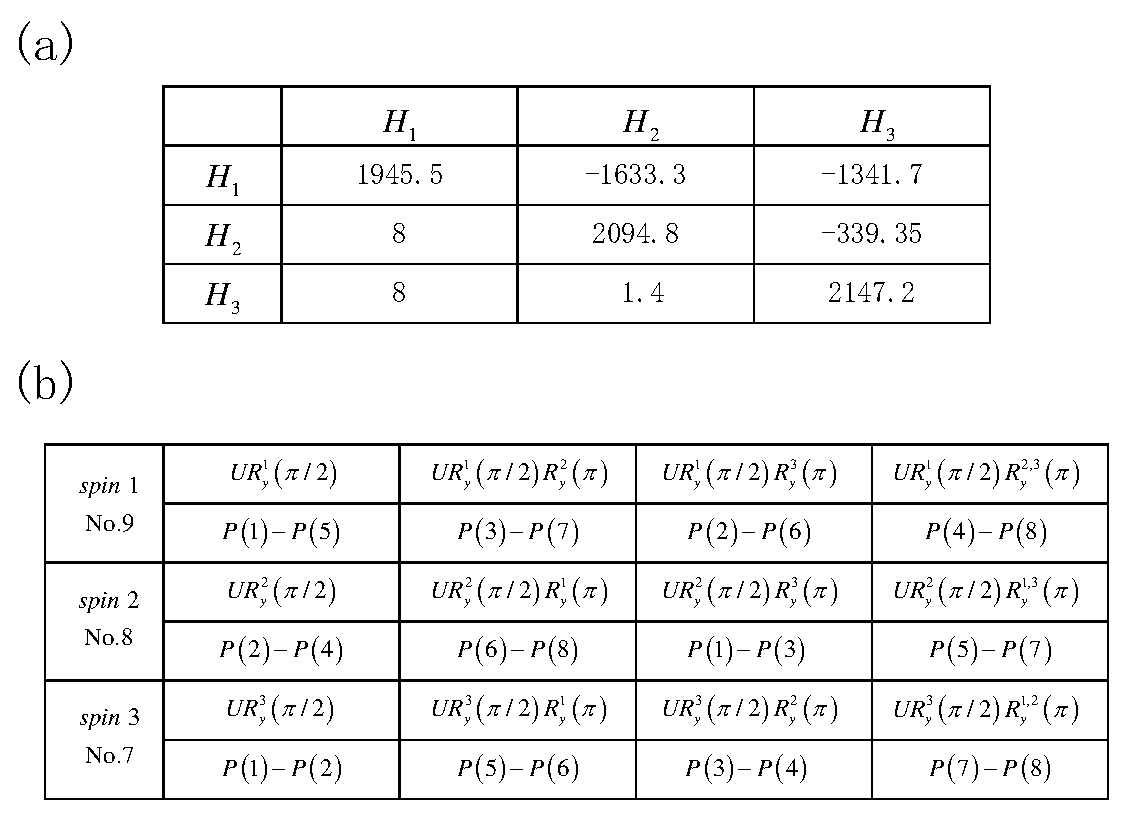
\includegraphics[width=0.9\columnwidth]{para.eps}
\caption{\footnotesize{(a) The parameters for fitting the spectrum of
1-Bromo-2,3-Dichlorobenzene (Hertz). The diagonal elements are chemical
shifts of the three protons, the upper-right off-diagonal elements
are dipolar coupling strengths while the lower-left ones are scalar
coupling strengths. (b) The read-out pulses and corresponding values
of $P(i)-P(j)$. The results are shown on the transitions of No.9, 8
and 7. Combined with the normalized condition $\sum_{i=1}^8P(i)=1$,
all the diagonal elements can be solved.}}\label{para}
\end{table}

\subsubsection*{\textbf{B. Populations' Measurement}}

With the system Hamiltonian confirmed, we consider the procedure of diagonalizing the Hamiltonian. It is not difficult to find a feasible unitary matrix $U$ to equalize
\begin{equation} \label{diag}
H_L = UH_SU^{\dag}
\end{equation}
where $H_S$ is the system Hamiltonian and $H_L$ is a diagonal
Hamiltonian, i.e., the Hamiltonian in the eigenbasis. Specially, for the
system Hamiltonian mentioned above, since U is not unique, we chose the transformation U as
\begin{eqnarray}\label{Transformation}
\left( {\begin{array}{*{20}c}
   {1} & {0} & {0} & {0} & {0} & {0} & {0} & {0}  \\
   {0} & {0.801} & {0.512} & {0} & {-0.303} & {0} & {0} & {0}  \\
   {0} & {0.375} & {-0.823} & {0} & {-0.420} & {0} & {0} & {0}  \\
   {0} & {0} & {0} & {0.810} & {0} & {0.126} & {0.559} & {0}  \\
   {0} & {-0.467} & {0.223} & {0} & {-0.856} & {0} & {0} & {0}  \\
   {0} & {0} & {0} & {0.458} & {0} & {-0.730} & {-0.508} & {0}  \\
   {0} & {0} & {0} & {0.344} & {0} & {0.672} & {-0.656} & {0}  \\
   {0} & {0} & {0} & {0} & {0} & {0} & {0} & {1}  \\ \nonumber
\end{array}} \right)
\end{eqnarray}
Through this labeling scheme all the transitions are
between two eigenstates from $\left\vert 000 \right\rangle_L$ to
$\left\vert 111 \right\rangle_L$ with $\left\vert 000
\right\rangle_L=\left\vert 000 \right\rangle_S,\left\vert 111
\right\rangle_L=\left\vert 111 \right\rangle_S$, where the
subscripts $L$ and $S$ represent the eigenbasis and computational basis. The
nine observable transitions in the thermal equilibrium spectrum are
marked in the transition diagram (Fig.\ref{energy_level}(c)).

\begin{figure}[h] \centering
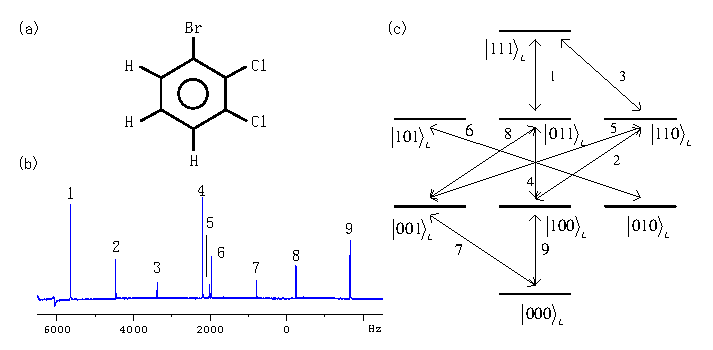
\includegraphics[width=\columnwidth]{energy_level.eps}
\caption{\footnotesize{(Color online)(a) Molecular structure of
1-Bromo-2,3-Dichlorobenzene in which the three protons form a 3-qubit
system. (b) Spectrum of the thermal equilibrium state
followed by a $\pi/2$ hard
pulse. All the observable transitions are labeled according to the descending
orders of the frequencies. (c) Diagram of corresponding
transitions in the eigenbasis. Only nine transitions are assigned. No.1 and No.9, No.2 and No.8, and
No.3 and No.7 lines express the transitions of qubit 1, 2 and 3 in
the $H_L$ picture, respectively.}}\label{energy_level}
\end{figure}

Without loss of generality, we focused on the right three
transitions No.7, 8 and 9. Considering a simple case that $\rho_S$
is a pure state $(\left\vert 000 \right\rangle\left\langle 000
\right\vert)_S$. In the isotropic weak-coupling liquid system, if the transition of qubit 1 is
excited (a selective pulse $R_y^1(\pi/2)$ is enough), a single peak
can be obtained in the spectrum. This is a universal way to test the
created pseudo pure state in liquid state NMR. However, in the
liquid-crystal system, a
single qubit rotation will not lead to a single peak but combination
of some relative peaks (see the right column of Fig.\ref{sim.eps}).
The complicated spectrum is obviously not convenient to read out the
information of density matrix. A straight idea to solve the problem
is to utilize the eigenbasis where the Hamiltonian is diagonal. From Eq (\ref{diag}) we can clearly see that adding the pulse of implementing transformation matrix $U$ after the read-out pulse in the sequence is suitable.
The right column of Fig.\ref{sim.eps} shows the spectra of
$(\left\vert 000 \right\rangle\left\langle 000 \right\vert)_S$ with
three read-out pulses
$UR_1^y(\pi/2),UR_2^y(\pi/2)R_3^y(\pi),UR_3^y(\pi/2)$. The second
pulse needs a $R_3^y(\pi)$ rotation as transition No.8 represents
$\left\vert 001 \right\rangle_L\rightarrow \left\vert 011
\right\rangle_L$, not $\left\vert 000 \right\rangle_L\rightarrow
\left\vert 010 \right\rangle_L$. The simulating spectra accord well
with the expected results, similarly to the liquid system.

\begin{figure}[h] \centering
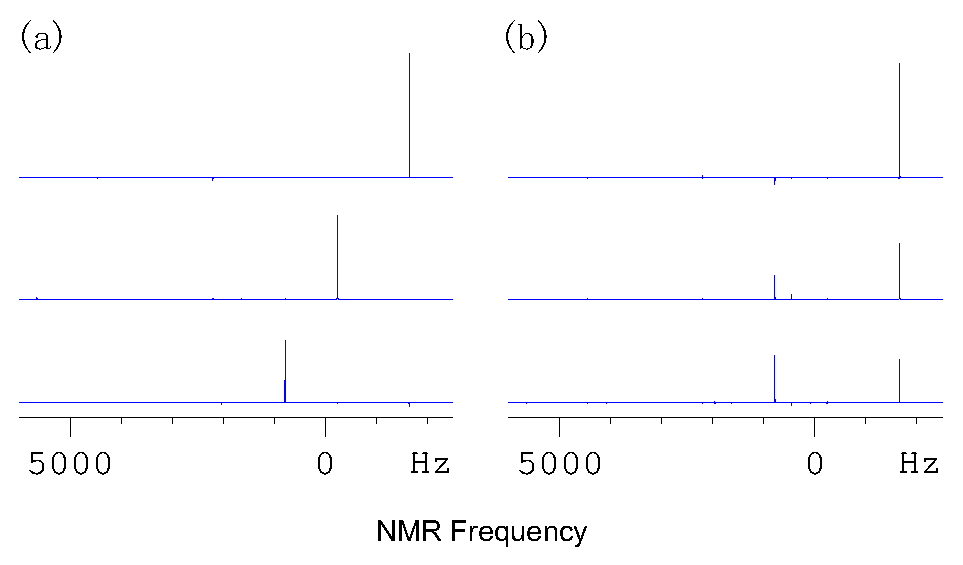
\includegraphics[width=\columnwidth]{sim.eps}
\caption{\footnotesize{(Color online) Simulation of the PPS's
observation. The left column (a) shows the spectra with the read-out
pulses $UR_1^y(\pi/2),UR_2^y(\pi/2)R_3^y(\pi),UR_3^y(\pi/2)$, while
the right (b) shows the spectra with the traditional read-out pulses
$R_1^y(\pi/2),R_2^y(\pi/2),R_3^y(\pi/2)$. We can see that the
spectra (a) are more comprehensible than those of
(b).}}\label{sim.eps}
\end{figure}

For reading-out the diagonal elements of a general density matrix
$\rho_S$, the method above is still effective. Defining the
populations of $(\left\vert 000 \right\rangle\left\langle 000
\right\vert)_S$ to $(\left\vert 111 \right\rangle\left\langle 111
\right\vert)_S$ are $P(1)$ to $P(8)$, $UR_1^y(\pi/2)$ would excite the
transitions $\left\vert 000 \right\rangle_L\rightarrow \left\vert
100 \right\rangle_L$ and $\left\vert 100 \right\rangle_L\rightarrow
\left\vert 000 \right\rangle_L$, displayed on transition No.9.
Through this transition, we can obtain
the value of $P(1)-P(5)$. Table. \ref{para} (b) shows all the
available values of $P(i)-P(j)$ through different read-out pulses.
Combined with the normalization condition $\sum_{i=1}^8P(i)=1$, all
the eight population values can be calculated. Now we have
accomplished the diagonal elements' tomography.


\subsubsection*{\textbf{C. Experiment}}

The experiment was divided into three steps: the psesudo-pure state
preparation, quantum random walk searching process, and populations'
measurement. Starting from the thermal equilibrium state, firstly we
need to create the PPS $\rho_{000}=\frac{1-\epsilon
}{8}\mathbf{1}+\epsilon \left\vert 000 \right\rangle \left\langle
000\right\vert$, where $\epsilon$ represents the polarization of the
system and $\mathbf{1}$ is the identity matrix. We used strongly
modulating pulses based on GRadient Ascent Pulse Engineering (GRAPE)
algorithm \cite{Khaneja,J. Baugh,C. A. Ryan} and gradient pulses to realize the PPS
preparation, with the numerical simulated fidelity 0.977. The top
spectrum of Fig. \ref{tomo} shows the experimental observation
of the PPS about the first qubit in the eigenbasis, which exhibits a
single absorption-shape peak if discarding the small errors.

The quantum random walk searching process contains two parts
actually: The preparation of initial state $|+\rangle^{\otimes3}$
($|+\rangle=(|0\rangle+|1\rangle)/\sqrt{2}$) and two times of
unitary evolution. We packed them together and calculated one GRAPE
pulse of 20ms and 250 segments whose fidelity is higher than 0.990 to
realize it. The reading-out operators listed in Table. \ref{para}
(b) are also performed when generating the GRAPE pulses of 20ms with
the fidelity 0.990. Four spectra observed on transition No.9 are
shown in Fig. \ref{tomo}. The
fidelity of the diagonal elements of the final density matrix is
0.983, with the probabilities of gaining $\left\vert 00
\right\rangle$, $\left\vert 01 \right\rangle$, $\left\vert
10 \right\rangle$, $\left\vert 11 \right\rangle$ being
0.513, 0.232, 0.197, 0.058. It demonstrates that we have completed
searching $\left\vert 00 \right\rangle$ based on the SKW
algorithm.



\begin{figure}[h] \centering
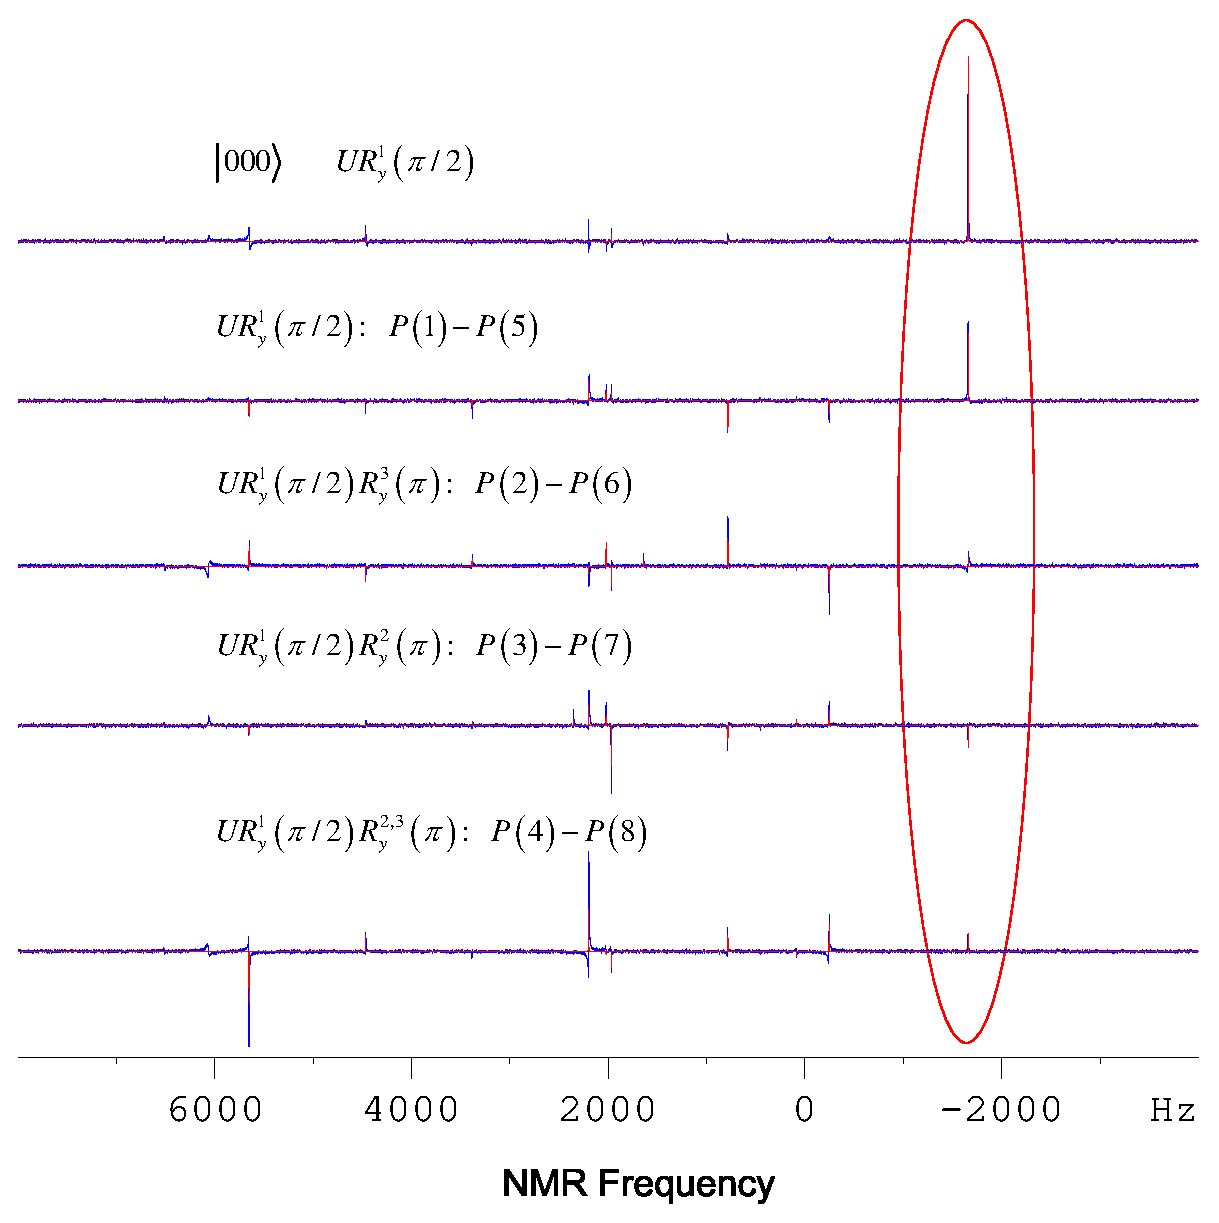
\includegraphics[width=\columnwidth]{tomo.eps}
\caption{\footnotesize{(Color online)One-dimensional NMR spectra
for measuring the diagonal elements of spin 1. The blue spectra are the experimental results, while the red spectra are the results by simulation.
As shown in Table. \ref{para} (b), we just concentrate on transition No.9
(marked by the ellipse) to read out $P(1)-P(5)$, $P(2)-P(6)$,
$P(3)-P(7)$ and $P(4)-P(8)$, with the four operators listed in the
figure. The top spectrum is the observation of the PPS $\left\vert
000 \right\rangle$, which is used as the benchmark. The theoretical
values of the four population-subtractions are 0.375, 0, -0.125,
0.125, while the experimental results are 0.383, 0.050, -0.061,
0.093.}}\label{tomo}
\end{figure}


Besides $\left\vert 00 \right\rangle$, we altered the target
states to $\left\vert 01 \right\rangle$, $\left\vert 10
\right\rangle$ and $\left\vert 11 \right\rangle$. The
experimental results of the SKW algorithm are plotted in Fig.
\ref{result}. It can be seen the experimental and theoretical
results are mostly consistent with little error.  The slight
difference between theory and experiment may be attributed to
decoherence, the RF field inhomogeneity and imperfect implementation of GRAPE pulses. The simulations are shown as the red spectra in Fig. \ref{tomo} to give the estimation of the credibleness of the experimental spectra.

\begin{figure}[h] \centering
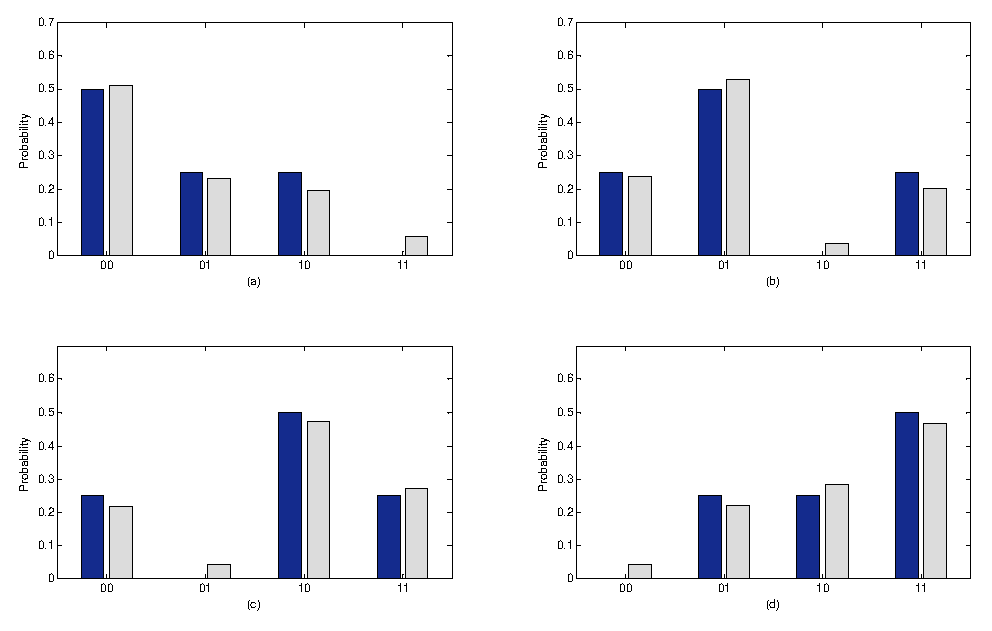
\includegraphics[width=\columnwidth]{result.eps}
\caption{\footnotesize{(Color online)Experimental results of the SKW algorithm.
(a), (b), (c), (d) correspond to the cases of
finding $\left\vert 00 \right\rangle_{12}$, $\left\vert 01
\right\rangle_{12}$, $\left\vert 10 \right\rangle_{12}$ and
$\left\vert 11 \right\rangle_{12}$. The blue bars represent the
theoretical prediction and the pray bars represent the experimental
analogue, respectively. }}\label{result}
\end{figure}

\subsection*{IV. Conclusion}

In summary, we experimentally implemented the search algorithm based
on the quantum random walk (the SKW algorithm) in the case of
1-out-of-4. This algorithm performs an oracle search on a database
of N items with $\emph{O}(\sqrt{\emph{N}})$ calls, having a speed-up
similar to the Grover's search algorithm. The experiment was carried
out on an NMR quantum information processor with strongly dipolar coupled spins. We used GRAPE pulses to realize
high-fidelity unitary operations and provided an effective way to
measure the diagonal elements of the density matrix with
one-dimensional NMR spectra. The experimental results agree well with the
theoretical expectations, which exhibit the superiority of the
algorithm.

This method is going to be extended to full tomography and higher qubits.  For further high-qubits, it becomes very challenging due to the complexity in the calculation of GRAPE pulses and diagonalization of the Hamiltonian.  However, as the speed and power of computers, and schemes of calculation advance these obstacles may be alleviated considerably in the near future.  Therefore, it, as in the case of  low-qubits, may still be a useful and effective method to test many interesting quantum algorithms and quantum information tasks.

\subsection*{Acknowledgement}

We thank Dieter Suter and Yiheng Lin for their help. This work was
supported by National Nature Science Foundation of China under Grant No. 10975124, Ministry
of Education of RPC, Chinese Academy of Sciences, the National Fundamental Research Program
2007CB925200.

$D_{ij}=-\frac{\miu_0}{4\pi}\frac{\gama^2h}{}$

\begin{thebibliography}{99}
\bibitem{Shor} P. W. Shor, SIAM J. Comput. \textbf{26}, 1484 (1997).
\bibitem{Grover} L. Grover,Phys. Rev. Lett. \textbf{79}, 325 (1997).
\bibitem{Farhi} Farhi E, Goldstone J, Gutmann S, Lapan J, Lundgren A, and Preda D, Science \textbf{292},412 (2001).
\bibitem{Aharonov} Y. Aharonov, L. Davidovich, and N. Zagury, Phys. Rev. A \textbf{48}, 1687 (1993).
\bibitem{Farhi and Gutmann} E. Farhi and S. Gutmann, Phys. Rev. A \textbf{58}, 915 (1998).
\bibitem{Ambainis and Back} A. Ambainis, E. Back, A. Nayak, A. Vishwanath, and J. Watrous, in \emph{Proceedings of the 30th
annual ACM Symposium on Theory of Computing} (Association for
Computing Machinery, New York, 2001), pp. 60-69.
\bibitem{Childs and Farhi} A. Childs, E. Farhi, and S. Gutmann, Quantum Inform. Process.
\textbf{1}, 35 (2002).
\bibitem{Childs and Cleve} A. Childs, R. Cleve, E. Deotto, E. Farhi, S. Gutmann, and D.
Spielman, Proc. 35th ACM Symposium on The- ory of Computing (STOC
2003), pp. 59-68.
\bibitem{Brun} T. A. Brun, H. A. Carteret and A. Ambainis, Phys. Rev. Lett. \textbf{91}, 130602 (2003).
\bibitem{Ambainis} A. Ambainis, SIAM J. Comput. \textbf{37}, 210 (2007).
\bibitem{Farhi and Goldstone} E. Farhi, J. Goldstone, and S. Gutmann, Theory Comput.
\textbf{4}, 169 (2008).
\bibitem{Childs} A. Childs, Phys. Rev. Lett. \textbf{102}, 180501 (2008).
\bibitem{Shenvi} N. Shenvi, J. Kempe and K. B. Whaley, Phys. Rev. A \textbf{67},
052307 (2003).
\bibitem{Ambainis and Kempe} A. Ambainis, J. Kempe, and A. Rivosh, \emph{Proceedings of the
16th ACM-SIAM SODA} (Society for Industrial and Applied
Mathematics, Philadelphia, 2005), pp. 1099�C1108.
\bibitem{Tulsi} A. Tulsi, Phys. Rev. A \textbf{78}, 012310 (2008).
\bibitem{Reitzner} D. Reitzner, M. Hillery, E. Feldman, and V. Bu$\check{z}$ek, Phys. Rev. A \textbf{79}, 012323 (2009).
\bibitem{Chandrashekar} C. M. Chandrashekar, R. Srikanth, and R. Laflamme, Phys.
Rev. A \textbf{77}, 032326 (2008).
\bibitem{Potocek} V. Poto$\check{c}$ek, A. G$\acute{a}$bris, T. Kiss and I. Jex, Phys.
Rev. A \textbf{79}, 012325 (2009).
\bibitem{Travaglione} B. C. Travaglione and G. J. Milburn, Phys. Rev. A \textbf{65},
032310 (2002).
\bibitem{Du} J. Du et al., Phys. Rev. A \textbf{67}, 042316 (2003).
\bibitem{Ryan} C. A. Ryan, M. Laforest, J. C. Boileau, and R. Laflamme,
Phys. Rev. A \textbf{72}, 062317 (2005).
\bibitem{Chandrashekar} C. M. Chandrashekar, Phys. Rev. A \textbf{74}, 032307 (2006).
\bibitem{Mahesh} T. S. Mahesh and D. Suter, Phys. Rev. A \textbf{74}, 062312 (2006).
\bibitem{Henry} M. K. Henry, C. Ramanathan, J. S. Hodges, C. A. Ryan, M. J. Ditty, R. Laflamme and D. G.Cory, Phys. Rev. Lett. \textbf{99}, 220501 (2007).
\bibitem{Zhang} J. Zhang, M. Ditty, D. Burgarth, C. A. Ryan, C. M. Chandrashekar, M. Laforest, O. Moussa, J. Baugh and R. Laflamme, Phys. Rev. A \textbf{80}, 012316 (2009).
\bibitem{Suryaprakash} N. Suryaprakash, Current Organic Chemistry \textbf{4}, 85-103, (2000).
\bibitem{Khaneja} N. Khaneja et al., J. Magn. Reson. \textbf{172}, 296 (2005);
\bibitem{J. Baugh} J. Baugh et al., Phys. in Can. \textbf{63}, No.4
(2007), 'Special issue on quntum information and quantum computing';
\bibitem{C. A. Ryan} C. A. Ryan et al., Phys. Rev. A \textbf{78}, 012328 (2008).

\end{thebibliography}

\end{document}
